\documentclass[conference]{IEEEtran}

\usepackage{amsmath}
\usepackage{amssymb}
\usepackage{graphicx}
% \usepackage{authblk}
\usepackage{float}
\usepackage{graphicx}
\usepackage[colorinlistoftodos]{todonotes}
\usepackage{soul}
\usepackage{algorithm}
\usepackage[noend]{algpseudocode}
\usepackage{subcaption}
%\usepackage[hyphenbreaks]{breakurl}
\usepackage[hyphens]{url}

%\graphicspath{ {c:/Users/mjutras/TeXworks/images/} }
\graphicspath{ {images/} }

% \author[6]{Deon Burchett, PhD}
% \author[5]{Brady Collea}
% \author[3]{Melanie Jutras}
% \author[2]{Les Servi, PhD}
% \author[1]{Randy Paffenroth, PhD}

% \affil[1,2,3,4]{The MITRE Corporation}
% \affil[5]{Worcester Polytechnic Institute}

\begin{document}

\title{Reducing Reporting Burden of Healthcare Data Using Robust Principal Component Analysis (RPCA)}
% My title isn't perfect but I think it is closer.  Let';s get it even better
%\title{Minimizing the Burden of Measuring Healthcare Data with Robust PCA}

\author{\IEEEauthorblockN{Les Servi}
\IEEEauthorblockA{The MITRE Corporation\\
202 Burlington Road \\ 
Bedford, MA 01730-1420 \\
Email: lservi@mitre.org}
\and
\IEEEauthorblockN{Randy Paffenroth}
\IEEEauthorblockA{Mathematical Sciences, Computer Science, \\
and Data Science\\
Worcester Polytechnic Institute\\
100 Institute Rd, \\
Worcester, MA 01609 \\
Email: rcpaffenroth@wpi.edu}
\and
\IEEEauthorblockN{Melanie Jutras,  Deon Burchett}
\IEEEauthorblockA{The MITRE Corporation\\
202 Burlington Road \\ 
Bedford, MA 01730-1420} 
}

\maketitle

% FIXME: Remove before submissions!  This is just to keep track of the length as we write.
\thispagestyle{plain}
\pagestyle{plain}
\todo{RCP: Remove page numbering before submission}

\begin{abstract}
The US government imposes reporting requirements on healthcare providers as health metrics are important for assessing and improving the US healthcare system.  However, proposed health metrics requirements can be unnecessarily burdensome if the preliminary analysis does not consider possible redundancies between the various metrics.  Accordingly, if some subset of the proposed metrics could be demonstrated to contain nearly all the information of  the full set of metrics,
% (e.g.,  having the subset permits one  to accurately predict the values of the metrics outside the subset)
then the reporting burden could be substantially  lightened with minimum impact.  However, such an analysis is complicated by anomalies in the collected metrics.  Accordingly, we propose a machine learning approach which simultaneously identifies redundancies in collected healthcare metrics and identifies anomalies in those collected metrics.
\end{abstract}

{\bf Keywords:} robust principal component analysis, anomaly
detection, health analytics, dimension reduction

\section{Introduction test}

\subsection{Background}
%\todo[color=yellow]{DONE: 8 Jul 2020:  This section was rewritten by LS.  I think it is in good shape but it would be nice for RP to quickly review it. }
Government agencies  mandate  metric reporting requirements to help them execute their missions.  In particular,  metrics are required for the evaluation of healthcare systems and initiatives in order to improve healthcare safety, quality and value. However, collecting and managing healthcare quality measures is expensive,  time consuming and prone to inaccuracies.  These inaccuracies take two forms.  Some inaccuracies are caused by the reality that attempts at precise metrics are not always met whereas others are wildly anomalous due to transcription errors, a misunderstanding of the precise requested metric or other business process errors.

A proposed set of health metrics may be unnecessarily large and onerous because the initial analysis to design the metrics did not properly account for redundancy of information between metrics.
%\todo[color=yellow,]{8 Jul  find details }Ref AcademyHealthAbstract]. 
Identifying such redundancies using standard methods revolving around computing correlations between the proposed metrics is hampered because the inevitable inaccuracies in the data will give a false sense of the correlations and underlying dimensionality of the metrics.   Instead, more advanced methods are required to effectively correct for imprecise inaccuracies in the data, identify and remove anomalous reported metrics, and only then examine the resulting correlations and dimensionality structure.

A promising data driven analytical approach to reduce metric reporting requirements burden without compromising the information which can be gleaned from the data is reported in this paper. This approach is applied to real data of  health metrics obtained from public use files collected over a period of one year.  However to validate the approach it was also applied to synthetic data where ground truth is known and both small errors and anomalous errors were intentionally inserted.


\subsection{Contribution}
This paper builds on previous Robust Principal Component Analysis (RPCA) research with an approach which is described and demonstrated to algorithmically remove anomalies as well as provide a low-rank approximation of the original data.  This low-rank approximation provides a pathway to reducing the reporting requirements with minimal adverse impact.  The details for the algorithms that underlie this work can be found in \cite{paffenroth2018robust,Paffenroth2012} (and references therein), and here we focus on the application of such algorithms to the particular nuances of healthcare metrics. 

In particular, empirical examples on synthetic data show that combining Sparse Principal Component Analysis (SPCA) with RPCA pre-processing was the only method tested herein that found all possible anomalies 
%and led to an MSE in reconstructing as low as possible. 
and correctly determined the minimum metric reporting burden. For example, we considered the case of $100$ training facilities and $100$ testing facilities with $20$ metrics each (but for which only $6$ would have sufficed). We complicated our task by adding $5$ anomalies in both  data sets.  

We detected, with no false alarms, all anomalies which permitted the algorithm to discover that the burden of measuring could have been reduced from $20$ metrics to only $6$ without \emph{any} appreciable loss of information.  

As shown in Figures \ref{fig:error_PCA_prediction_without_RPCA}, \ref{fig:error_PCA_prediction_with_RPCA_first}, \ref{fig:error_SPCA_prediction_without_RPCA_first}, and \ref{fig:error_SPCA_prediction_without_RPCA_first_selected} competing methods either mis-detect the anomalies, incorrectly predict the non-anomalous entries, or get the required number of required metrics incorrect.
As shown in Figures \ref{fig:error_SPCA_prediction_with_RPCA_first} and \ref{fig:error_SPCA_prediction_with_RPCA_first_selected} our method can be seen to be the only method that accomplishes all three tasks (anomaly detection, correctly computing the number of required metrics, and reconstructing the complete data set).
\todo{RCP: Mention real data set here one real data metrics are done.}
%\todo[inline, color = yellow] {What do we do with this reference to newPaper?  RCP DONE!  I used my original RPCA paper and our arxiv.org paper.   If, however, you mean the upcoming that has not even been started yet, I don't think that we can cite it. }
\todo{RCP:  Make punchier and more quantitative, e.g. "In particular, empirical examples show it found XX more anomalies, and led to XX better MSE in reconstructing original dataset. RCP needs to write some code and redo some runs to get MSE numbers}
\todo{RCP:  Add something about what made the synthetic problem hard, eg, N anomolous (M percent) which are on average size Y as well as noise of size Z thrown in.}
\todo[color=red]{RCP and LS:  Need to nail down this request "Also, need a sentence about real data: Had a method to verify that it was catching anomalies and also showed that it appeared that we can reduce the metric burden by X with minimal impact."}


In this paper we make several contributions, including

\begin{itemize}
    \item we demonstrate how RPCA can be used to find anomalies in both real and synthetic data sets,
    \item we show how, once anomalies are identified, one may identify a small subset of predictors from which the remaining predictors may be generated, and
    \item we apply these algorithms to a real-world healthcare data set to robustly select a subset of predictors that may be cheaply measured and detect anomalies in testing data.
\end{itemize}

\section{Analysis}

In contrast, data analysis was performed on both synthetic and real world data sets which will be described in the sections below. Analysis of synthetic data is particularly useful as we know the ground truth. Analysis of real world data sets is complicated by the fact that in many cases, we do not know ground truth.  This can make anomaly detection and dimension reduction difficult as we do not know what the outlier data points are and we also do not know the true rank of the data.


% \todo{should include bullet list}
% TBD TBD TBD TBD TBD TBD TBD TBD TBD TBD TBD TBD TBD TBD TBD TBD
% TBD TBD TBD TBD TBD TBD TBD TBD TBD TBD TBD TBD TBD TBD TBD TBD
% TBD TBD TBD TBD TBD TBD TBD TBD TBD TBD TBD TBD TBD TBD TBD TBD
% TBD TBD TBD TBD TBD TBD TBD TBD TBD TBD TBD TBD TBD TBD TBD TBD
% TBD TBD TBD TBD TBD TBD TBD TBD TBD TBD TBD TBD TBD TBD TBD TBD

% \begin{itemize}
% \item TBD TBD TBD TBD TBD TBD TBD TBD TBD TBD TBD TBD TBD TBD TBD TBD
% TBD TBD TBD TBD TBD TBD TBD TBD TBD TBD TBD TBD TBD TBD TBD TBD
% \item TBD TBD TBD TBD TBD TBD TBD TBD TBD TBD TBD TBD TBD TBD TBD TBD
% TBD TBD TBD TBD TBD TBD TBD TBD TBD TBD TBD TBD TBD TBD TBD TBD
% \item TBD TBD TBD TBD TBD TBD TBD TBD TBD TBD TBD TBD TBD TBD TBD TBD
% TBD TBD TBD TBD TBD TBD TBD TBD TBD TBD TBD TBD TBD TBD TBD TBD
% \end{itemize}

\section{Background}
\subsection{Traditional PCA} \label{PCA}
\todo[color=yellow]{LS:  Update code to reflect that it is not true that the main concern about PCA is the difficulty to interpret.  We don't like PCA because it reduces the dimension of the data but it doesn't reduce the number of measurements we use.}
\todo[color=yellow]{LS:  It would be great to work through this section since it was copied from our arxiv.org paper.  This is a different audience and we want to avoid self-plagarism.}
Traditional Principal Components Analysis (PCA) works well for dimensionality reduction.  However, it is often seen as difficult to interpret.  The reason for this is that PCA produces a set of results which are a linear combination of features.  This is useful for understanding the rank or underlying dimension, but does not help to select specific measures from a set of attributes. Additionally, and an important note for this research, is that PCA is extremely sensitive to outliers.  One outlier in the data can completely change the results.

In particular, consider a collection of
points $\{x_0,...,x_m\}$ with $x_i \in \mathbb{R}^n$.  Following the notation and presentation in \cite{paffenroth2018robust} we note that each point represents some object of interest, for example the $n$ measured properties of some health-care provider, the set of points $\{x_0,...,x_m\}$ would therefore
represent the collection of health-care providers that we intend to analyze.
The goal of PCA is therefore to compute a linear projection of the points $\{x_0,...,x_m\}$ into a new
set of points $\{\hat{x}_0,...,\hat{x}_m\}$ that each lie on some $k$-dimensional subspace of the original
$n$-dimensional space.  

The idea is that the subspace is chosen such that each point $x_i$ has to be moved as little as possible
to make it lie on the $k$-dimensional subspace.  If one encodes the measurement $x_i$ into a matrix
$X \in \mathbb{R}^{m \times n}$ with each $x_i$ being a row of $X$, then one can find
the low-dimensional representation $X$ by solving an optimization problem such as 

\begin{align} \label{PCAopt}
  &\min_{L} \| L-X \|_F^2 \\ \nonumber
  \text{subject to}\quad & \rho(L) \le k
\end{align}

\noindent where $\| L-X \|_F^2$ is the sum of the squares of the entries of $L-X$ (often called the Frobenius norm), $L \in \mathbb{R}^{n \times m}$ and $\rho(L)$ is the \emph{rank} of $L$ (the dimension of the subspace spanned by the rows of $L$).

The optimization problem in (\ref{PCAopt}) is often solved by way of the Singular Value
Decomposition (SVD) \cite{Eckart1936}.  In particular, by the SVD we know that $X=U \Sigma V^T$ where, assuming that $n<m$, we have $U \in \mathbb{R}^{m \times n}$ and $U$ is unitary in that $U^T U = I$; $V \in \mathbb{R}^{n \times n}$ and $V$ is unitary in that $V^T V = I$; and $\Sigma \in \mathbb{R}^{n \times n}$ and $\Sigma$ is diagonal with positive diagonal entries $\sigma_i$ called the \emph{singular values} of $X$.

Further, assuming the singular values are ordered such that $\sigma_i \ge \sigma_{i+1}$
and, for a given matrix $X$, we denote by $X_{i:j,k:l}$ the principle sub-matrix of $X$ comprised of rows $i$ through $j$ and columns $k$ through $l$, one can write principle component analysis as 

\begin{align*}
X 
& = 
\begin{bmatrix}
U_{1:k,1:k} & U_{1:k,k+1:m} \\
U_{k+1:n,1:k} & U_{k+1:n,k+1:m} \\
\end{bmatrix}
\begin{bmatrix}
\Sigma_{1:k,1:k} & 0 \\
0 & \Sigma_{k+1:n,k+1:n} \\
\end{bmatrix}
\begin{bmatrix}
V_{1:k,1:k} & V_{1:k,k+1:n} \\
V_{k+1:n,1:k} & V_{k+1:n,k+1:n} \\
\end{bmatrix} \\
\end{align*}

\noindent Now, by assumption, every entry of $\Sigma_{k+1:n,k+1:n}$ is smaller than the smallest
entry of $\Sigma_{1:k,1:k}$ we approximate $X$ by setting $\Sigma_{k+1:n,k+1:n}=0$
and get

\begin{align*}
& X \approx 
\begin{bmatrix}
U_{1:k,1:k} & U_{1:k,k+1:m} \\
U_{k+1:n,1:k} & U_{k+1:n,k+1:m} \\
\end{bmatrix}
\begin{bmatrix}
\Sigma_{1:k,1:k} & 0 \\
0 & 0 \\
\end{bmatrix}
\begin{bmatrix}
V_{1:k,1:k} & V_{1:k,k+1:n} \\
V_{k+1:n,1:k} & V_{k+1:n,k+1:n} \\
\end{bmatrix} \\
& = 
\begin{bmatrix}
U_{1:k,1:k} & 0 \\
U_{k+1:n,1:k} & 0 \\
\end{bmatrix}
\begin{bmatrix}
\Sigma_{1:k,1:k} & 0 \\
0 & 0 \\
\end{bmatrix}
\begin{bmatrix}
V_{1:k,1:k} & V_{1:k,k+1:n} \\
0 & 0 \\
\end{bmatrix} \\
& = 
\begin{bmatrix}
U_{1:k,1:k} \\
U_{k+1:n,1:k} \\
\end{bmatrix}
\begin{bmatrix}
\Sigma_{1:k,1:k}
\end{bmatrix}
\begin{bmatrix}
V_{1:k,1:k} & V_{1:k,k+1:n} \\
\end{bmatrix} \\
& = \hat{U} \hat{\Sigma} \hat{V}^T
\end{align*}

We observe that if $X$ is exactly of rank $k$ then equality in the above equation holds (since $\Sigma_{k+1:n,k+1:n}=0$ is already true).  Similarly, we also have that $\hat{U} \hat{\Sigma} \hat{V}^T$ is the optimal low-rank approximation of $X$.  So, $X$ can we compressed to $k$ predictors by computing $X \begin{bmatrix} V_{1:k,1:k} & V_{1:k,k+1:n} \\ \end{bmatrix}^T$ and reconstructed by using $(X \begin{bmatrix} V_{1:k,1:k} & V_{1:k,k+1:n} \\ \end{bmatrix}^T) \begin{bmatrix} V_{1:k,1:k} & V_{1:k,k+1:n} \\ \end{bmatrix}$

\todo{RCP:  Maybe wrong level of detail above.  Check later.}

Unfortunately, in the current context, PCA has two important deficiencies.  First, while PCA effectively compresses the input measurements, each of the $k$ principal components in general depends on all of the $n$ original measurements.   As we are interested in not having to measure all $n$, but rather a subset, we note that if $X$ is of exactly rank $k$ the any $k$ columns of $X$ can be used to reconstruct the other $n-k$ columns of $X$.
\todo{RCP:  Maybe more detail here.  Check later.}
%TBD TBD TBD TBD TBD TBD TBD TBD TBD TBD TBD TBD TBD TBD TBD TBD TBD TBD TBD TBD TBD TBD TBD TBD TBD TBD TBD TBD TBD TBD TBD TBD TBD TBD TBD TBD TBD TBD TBD TBD.  
Second, the data sets that we wish to analyze likely have outliers that are not actually part of the true representation of the data.  Unfortuantely, the squared error in (\ref{PCAopt}) tends to introduce large inaccuaries in the SVD of $X$ if $X$ contains anomalies.
\todo{RCP:  Maybe more detail here.  Check later.}
%TBD TBD TBD TBD TBD TBD TBD TBD TBD TBD TBD TBD TBD TBD TBD TBD TBD TBD TBD TBD TBD TBD TBD TBD TBD TBD TBD TBD TBD TBD TBD TBD TBD TBD TBD TBD TBD TBD TBD TBD.  
Accordingly, we require a version of PCA what is robust to these types of measurement anomalies.   Fortunately, Robust Principal Component Analysis (RPCA) \cite{Candes2009,
 Candes2011, Chandrasekaran2009, Cai2010, Paffenroth2012a,Paffenroth2013b} provides precisely the type of approach that we require.   

\subsection{Sparse PCA}\label{SPCA}

As opposed to PCA, in which the principal components are generally linear combinations of all of the predictors, one can instead consider Sparse PCA \cite{htf01} in which individual predictors are chosen to reconstruct the rest. In particular, if $X$ is exactly of rank $k$ then any $k$ columns of $X$ can be used to exactly reconstruct the remaining $n-k$ columns of $X$.

% TBD TBD TBD TBD TBD TBD TBD TBD TBD TBD TBD TBD TBD TBD TBD TBD TBD TBD TBD TBD TBD TBD TBD TBD TBD TBD TBD TBD TBD TBD TBD TBD TBD TBD TBD TBD TBD TBD TBD TBD.TBD TBD TBD TBD TBD TBD TBD TBD TBD TBD TBD TBD TBD TBD TBD TBD TBD TBD TBD TBD TBD TBD TBD TBD TBD TBD TBD TBD TBD TBD TBD TBD TBD TBD TBD TBD TBD TBD TBD TBD.TBD TBD TBD TBD TBD TBD TBD TBD TBD TBD TBD TBD TBD TBD TBD TBD TBD TBD TBD TBD TBD TBD TBD TBD TBD TBD TBD TBD TBD TBD TBD TBD TBD TBD TBD TBD TBD TBD TBD TBD.

For example, consider $S$ is a selection matrix with $S \in \{0,1\}^{n \times K}$ and every column of $S$ has precisely a single entry of $1$ and every row of $S$ has at most a single entry of $1$.

For example

$$
S = 
\begin{bmatrix}
1 & 0 & 0 \\
0 & 0 & 0 \\
0 & 1 & 0 \\
0 & 0 & 1 \\
0 & 0 & 0 \\
0 & 0 & 0 \\
\end{bmatrix}
$$

Selects the $1$-st, $3$-rd and $4$-th column of an $X$ that originally had $6$ columns.

So, in general we write 

$$X_K = X S$$

for selecting $k$ columns from $X$.

If were to estimate $X$ from $X_K$ we would need two properties.

First, our estimate $\hat{X}$ of $X$ should have the property that it agrees with $X$ on $S$, in other words there is some $Z$ such that

$$
\hat{X} = X S S^T + Z (I-S S^T) = X_K S^T + Z (I-S S^T)
$$

Second, our estimate $\hat{X}$ must lay on the subspace spanned by singular vectors of $X$.  Equivalently, we need that

$$
\hat{X} = \hat{X} V V^T.
$$

Plugging the first into the second we get

$$
X_K S^T + Z (I-S S^T) = (X_K S^T + Z (I-S S^T)) V V^T 
$$

expanding we get 

$$
X_K S^T + Z (I-S S^T) = X_K S^T V V^T + Z (I-S S^T)V V^T
$$

Collecting terms

$$
X_K (S^T - S^T V V^T) = Z ((I-S S^T)V V^T - (I-S S^T))
$$

which we can solve for $Z$ and \emph{only depends on $X_K$}.

\subsection{Robust PCA Convex Optimization Approach}
The Convex Optimization approach is based on Robust Principal Component Analysis (RPCA). In this section we closely follow the notation in \cite{Paffenroth2012a,Paffenroth2013b,paffenroth2018robust}. The RPCA approach will both remove anomalies and provide a low rank approximation of the original data. This is accomplished with a combination of a nuclear norm and a one norm which is regularized by a tuning parameter, $\lambda$ to induce sparsity. The Robust PCA formulation is as follows.

\begin{align} \label{RPCA}
  &\min_{L,S}\rho(L)+\lambda\|S\|_{0}\\ \nonumber
  \qquad \text{subject to} \quad &
                                   |X-(L+S)| = 0
\end{align}

\todo[color=yellow]{LS:  Needs to be rewritten since it is copied from the arxiv paper}
% FIXME Copied from arxiv paper
%%%%%%%%%%%%%%%%%%%%%%%%%%%%%%%%%%%%%%%%%%%%%%%%%%%%%%%%%%%%%%%%%%%%%%%%
\noindent where $\rho(L)$ is the rank of $L$, $\|S\|_{0}$ is the
number of non-zero entries in $S$, and $\lambda$ is a coupling
constant which controls the trade-off between the low-rank matrix $L$
and the sparse matrix $S$.  Unfortunately, as opposed to
\eqref{PCAopt}, we do not have any closed form solution to
\eqref{RPCA}.   Even worse, a n\"{a}ive, brute force
approach to the problem, where one searches over all possible
combinations of low-rank matrices $L$ and entries of $S$ corresponding
to a presupposed number of anomalies, would be NP-hard in the number
of anomalies.

However, Theorem 1.2 in \cite{Candes2011}, Theorem 2.1
\cite{Paffenroth2012a}, and many similar theorems in the extant
literature provide remarkable guarantees for recovery $L$ and $S$.
Providing details for these theorems would take us too far afield in
the current context, and the interested reader may refer to extant
literature for details \cite{Candes2009, candes09ex, Chandrasekaran2009,
  Candes2011, Paffenroth2012a, Paffenroth2013b}.
Herein we merely observe that the optimization in \eqref{RPCA} is
NP-hard, but a closely related problem can be solved if some technical
conditions are met.\footnote{Classically, these conditions bound the
  rank of $L$, bound the sparsity of $S$, require that the columns of
  $L$ are \textit{incoherent} far from the standard basis, and require
  that the non-zero entries in $S$ are distributed uniformly.}

In particular, assuming such conditions are met, then, with high
probability the \emph{convex} program

\begin{align} \label{mainalg}
  &\min_{L,S}\|L\|_{*}+\lambda\|S\|_{1}\\ \nonumber
  \qquad \text{subject to} \quad &
                                   |Y-(L+S)|
                                   \preceq \epsilon
\end{align}

\noindent recovers $L$ and $S$, where
$\|L\|_{*} = \sum_{i=1}^m\sigma_{i}$ is the nuclear norm of $L$ (i.e.,
the sum of the singular values of $L$) and
$\|S\|_1:= \sum_{ij}|S_{ij}|$.  $\lambda$ is as in \eqref{mainalg} and
$\epsilon$ is a set of point-wise error constraints which we used to
ameliorate the noise found in real-world data.  The reader familiar
with such algorithms will no-doubt note that $\|S\|_1$ is a convex
relaxation of $\|S\|_0$, and $\|L\|_*$ is a convex relaxation of
$\rho(L)$, and such problems can be efficiently solved
\cite{Boyd2010a, Candes2009, Candes2011, Paffenroth2012a,
  Paffenroth2013b, Halko2011}.

Note, in \eqref{mainalg}, the importance of the parameters $\lambda$
and $\epsilon$.  In particular, Theorem 1.2 in \cite{Candes2011}
proves that setting $\lambda = \frac{1}{\sqrt{\max(m,n)}}$, where
$Y \in \mathbb{R}^{m \times n}$ guarantees the \emph{recovery} of $L$
and $S$ from $Y$ (assuming the constraints mentioned previously).
% FIXME Copied from arxiv paper
%%%%%%%%%%%%%%%%%%%%%%%%%%%%%%%%%%%%%%%%%%%%%%%%%%%%%%%%%%%%%%%%%%%%%%%%

Approximation methods are used as implemented in the dimredu python package and available as open source here
\todo[color=red]{RCP and LS:  We need to discuss... RCP is not sure what this means "What about the results from Melanie et al.?"}
\footnote{The Python libraries and Jupyter notebook for generating the results in this paper can be found on bitbucker.org at ANONYMOUS.}

% \subsubsection{Robust PCA Combinatorial Approach}
% \todo[color=yellow,inline]{Ok, this is important.  We are not actually doing any Sparse PCA!?   This indicates we are just doing Robust PCA.   That does agree with my memory, now that I think about it.  This makes things easier, but I am not sure what the combinatorial approach is anymore.}
% \todo[inline]{Insert Deon's Problem Formulation here}

\section{Data: Synthetic and real-world}

\subsection{Synthetic Data}

Creation of synthetic data relies upon the following variables :
\begin{itemize}
\item $m$: total number of samples
\item $n$: total number of features 
\item $k$: number of independent features
\item $numAnoms$: number of anomalies in the data
\item $sizeAnom$: size of each anomaly
\item $noiseSize$: standard deviation of $0$-mean Gaussian noise added to each element of the matrix 
\end{itemize}

Based upon the above variable definitions, a synthetic data matrix $X$ is then created using the following steps
\begin{enumerate}
\item Initially, two matrices $A \in \mathbb{R}^{m \times k}$ and $B \in \mathbb{R}^{k \times n}$ are constructed and a low-rank matrix $L$ is constructed by setting $L = AB$.
%\todo{DONE: LS: Are U and V unitary?  If so, we shoudl state this.  RCP: No, and I have updated the notation to make this more clear.}
\item An anomaly matrix $S$ of the same size as $L$ is constructed.  Each of the entries of $S$ is $0$ except for $numAnoms$ entries, selected uniformly at random, which are set to $sizeAnoms$.
\item A noise matrix $N$ of the same size as $L$ is constructed. Each of the entries of $N$ is set to a random draw from a Gaussian distribution with mean $0$ and standard deviation $noiseSize$.
\end{enumerate}
\noindent Our final synthetic $X$ matrix is then constructed as $X=L+S+N$.  In particular, this model is faithful to our health data since it is a combination of low-rank ambient data and sparse anomalies, as we expect in real-world hospital data.
\todo{RPC: Needs more here. Check later.}
% TBD TBD TBD TBD TBD TBD TBD TBD TBD TBD TBD TBD TBD TBD TBD TBD TBD TBD TBD TBD TBD TBD TBD TBD TBD TBD TBD TBD TBD TBD TBD TBD TBD TBD TBD TBD TBD TBD TBD TBD.TBD TBD TBD TBD TBD TBD TBD TBD TBD TBD TBD TBD TBD TBD TBD TBD TBD TBD TBD TBD TBD TBD TBD TBD TBD TBD TBD TBD TBD TBD TBD TBD TBD TBD TBD TBD TBD TBD TBD TBD.TBD TBD TBD TBD TBD TBD TBD TBD TBD TBD TBD TBD TBD TBD TBD TBD TBD TBD TBD TBD TBD TBD TBD TBD TBD TBD TBD TBD TBD TBD TBD TBD TBD TBD TBD TBD TBD TBD TBD TBD.

% \subsubsection{Add Noise}
% Some of our experiments were performed on clean synthetic data as a base, while other experiments included the addition of noise. Our method for adding noise to the data was as follows. SciPy's numpy random package was used to draw random samples from a Gaussian distribution mean centered at zero with a standard deviation equal to 0.1 times the standard deviation of the clean matrix $X$ described in previous sections. The line of python code to accomplish this task is as follows.\\\\
% $noise = np.random.normal(0, 0.1*np.std(myX), myX.shape)$
% \subsubsection{Add Anomalies}
% For the purpose of our experiments, many different input files were created with varying number of anomalies as well as anomalies that were various magnitudes. The method for adding anomalies to the data was as follows.
% \begin{itemize}
% \item Randomly select a cell in the matrix
% \item Make sure an anomaly has not already been added at this location
% \item Randomly decide if we're inserting a positive or negative anomaly
% \item Insert the anomaly of size $sizeAnom$ with the randomly generated sign at the randomly selected location
% \end{itemize}

\subsection{Real Data}

The health data set that we chose to analyze was provided by the Centers for Medicare and Medicaid Services (CMS). The public use file is available at CMS.gov and contains data related to the Shared Savings Program Accountable Care Organizations (ACO) in the year 2016. The dataset consists of 432 ACOs and makes use of 34 nationally recognized Quality Measures.  A simple boxplot visualization of the normalized dataset reveals the distributions as shown in Figure \ref{fig:boxall}, skewed data and outliers of the various features. It is not unusual for real world data to be noisy and impacted by outliers due to human error, but it does complicate analysis.\\

\begin{figure}[H]
    \centering
    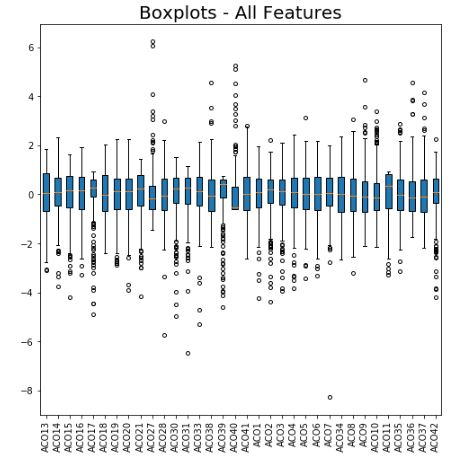
\includegraphics{BoxPlots_ALL.jpg}
    \caption{Boxplot of all features}
    \label{fig:boxall}
\end{figure}
%\todo{RCP: DONE. Maybe that part of the paper should be summarized and some or all of these figures deleted.}
\todo[color=yellow]{LS:  Add more explaination of analysis of these predictors.  This is the part where we get to call this a healthcare paper.}

The quality measures can be divided into distinct sub-categories. 
%Boxplots created for each of these categories may reveal differences in the data distributions for each category of features. The GPRO features in particular appear to have greater variability and larger outliers as shown in \ref{fig:boxgpro}.

\begin{enumerate}
\item GPRO - Group Practice Reporting Option Features (16 measures) : GPRO features are collected by a web interface which was designed specifically to capture ACO-reported clinical quality data.

% \begin{figure}[H]
%     \centering
%     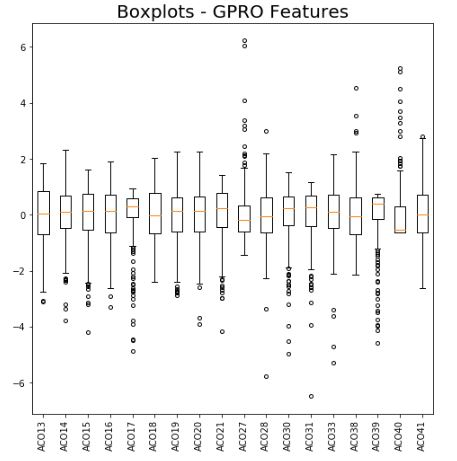
\includegraphics{BoxPlots_GPRO.jpg}
%     \caption{Boxplot of GPRO features}
%     \label{fig:boxgpro}
% \end{figure}


\item CAHPS - Consumer Assessment of Healthcare Providers Features (10 measures) : CAHPS features, as shown in \ref{fig:boxcahps}, are collected by a survey administered by a CMS-approved vendor selected and paid for by individual ACOs.

% \begin{figure}[H]
%     \centering
%     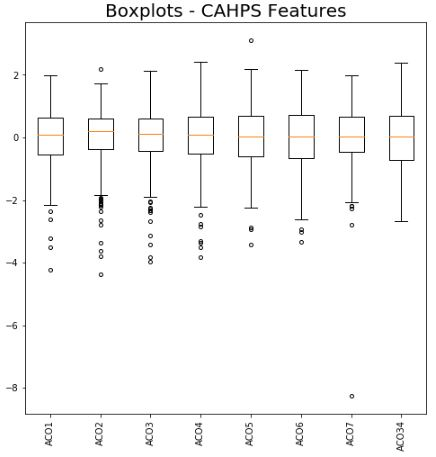
\includegraphics{BoxPlots_CAHPS.jpg}
%     \caption{Boxplot of CAHPS features}
%     \label{fig:boxcahps}
% \end{figure}

\item EHR - Electronic Health Record Features (8 measures) : EHR features, as shown in Figure \ref{fig:boxehr}, are calculated by the CMS ACO PAC based on CMS claims and administrative data extracted from the National Level Repository. 
\end{enumerate}

% \begin{figure}[H]
%     \centering
%     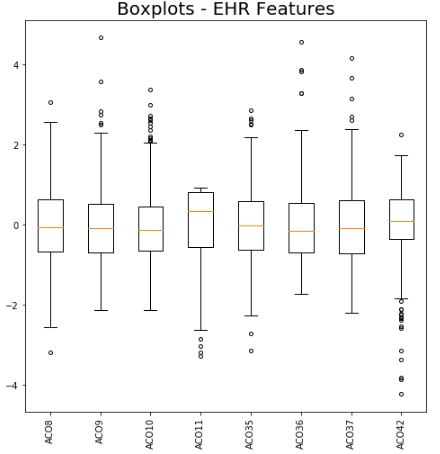
\includegraphics{BoxPlots_EHR.jpg}
%     \caption{Boxplot of EHR features}
%     \label{fig:boxehr}
% \end{figure}



\section{Experimental procedure}
In our experiments we follow the following test protocol to compare the following four competing methods
\todo{RCP: Add more detail here: This is the big idea of the approach}
\begin{itemize}
    \item Using PCA to make predictions from linear combinations of the original predictors as in Section~\ref{PCA}.
    \item Using SPCA to make predictions from a subset of the original predictors as in Section~\ref{SPCA}.
    \item Perform RPCA first and the use PCA to make predictions from linear combinations of the columns of $L$ as in Section~\ref{PCA}.
    \item Perform RPCA first and the use SPCA to make predictions from a subset of the columns of $L$ as in Section~\ref{SPCA}.
\end{itemize}

Each of these procedures are detailed in the following section.

%TBD TBD TBD TBD TBD TBD TBD TBD TBD TBD TBD TBD TBD TBD TBD TBD TBD TBD TBD TBD TBD TBD TBD TBD TBD TBD TBD TBD TBD TBD TBD TBD TBD TBD TBD TBD TBD TBD TBD TBD.TBD TBD TBD TBD TBD TBD TBD TBD TBD TBD TBD TBD TBD TBD TBD TBD TBD TBD TBD TBD TBD TBD TBD TBD TBD TBD TBD TBD TBD TBD TBD TBD TBD TBD TBD TBD TBD TBD TBD TBD.TBD TBD TBD TBD TBD TBD TBD TBD TBD TBD TBD TBD TBD TBD TBD TBD TBD TBD TBD TBD TBD TBD TBD TBD TBD TBD TBD TBD TBD TBD TBD TBD TBD TBD TBD TBD TBD TBD TBD TBD.

\subsubsection{Approach}

%TBD TBD TBD TBD TBD TBD TBD TBD TBD TBD TBD TBD TBD TBD TBD TBD TBD TBD TBD TBD TBD TBD TBD TBD TBD TBD TBD TBD TBD TBD TBD TBD TBD TBD TBD TBD TBD TBD TBD TBD.TBD TBD TBD TBD TBD TBD TBD TBD TBD TBD TBD TBD TBD TBD TBD TBD TBD TBD TBD TBD TBD TBD TBD TBD TBD TBD TBD TBD TBD TBD TBD TBD TBD TBD TBD TBD TBD TBD TBD TBD.TBD TBD TBD TBD TBD TBD TBD TBD TBD TBD TBD TBD TBD TBD TBD TBD TBD TBD TBD TBD TBD TBD TBD TBD TBD TBD TBD TBD TBD TBD TBD TBD TBD TBD TBD TBD TBD TBD TBD TBD.

\todo{RCP: Perhaps these can be combined to make things shorter if we need space.}

In detail, the algorithm for our approach is the following when we use PCA by itself.  
%TBD TBD TBD TBD TBD TBD TBD TBD TBD TBD TBD TBD TBD TBD TBD TBD TBD TBD TBD TBD TBD TBD TBD TBD TBD TBD TBD TBD TBD TBD TBD TBD TBD TBD TBD TBD TBD TBD TBD TBD.TBD TBD TBD TBD TBD TBD TBD TBD TBD TBD TBD TBD TBD TBD TBD TBD TBD TBD TBD TBD TBD TBD TBD TBD TBD TBD TBD TBD TBD TBD TBD TBD

\begin{algorithm}
\caption{PCA prediction}\label{alg:pca prediction}
\begin{algorithmic}[1]
\Procedure{PCA prediction}{$X_{train}, X_{test}$}
\State Perform PCA to get $U \Sigma V^T = SVD(X_{train})$
\State Project $X_{test}$ as $L_{test} = X_{test} V V^T$
\State Anomalies are $S_{test} = X_{test} - L_{test}$
\State \textbf{return} $L_{test}$, $S_{test}$
\EndProcedure
\end{algorithmic}
\end{algorithm}

In detail, the algorithm for our approach is the following when we use SPCA by itself.
% TBD TBD TBD TBD TBD TBD TBD TBD TBD TBD TBD TBD TBD TBD TBD TBD TBD TBD TBD TBD TBD TBD TBD TBD TBD TBD TBD TBD TBD TBD TBD TBD TBD TBD TBD TBD TBD TBD TBD TBD.TBD TBD TBD TBD TBD TBD TBD TBD TBD TBD TBD TBD TBD TBD TBD TBD TBD TBD TBD TBD TBD TBD TBD TBD TBD TBD TBD TBD TBD TBD TBD TBD

\begin{algorithm}
\caption{SPCA prediction}\label{alg:spca prediction}
\begin{algorithmic}[1]
\Procedure{SPCA prediction}{$X_{train}, X_{test}$}
\State Make a selection matrix $S_{sel}$
\State Select $k$ columns of $X_{train}$ to get $X_k = X_{train} S_{sel}$
\State Perform PCA to get $U \Sigma V^T = SVD(X_k)$
\State Solve for $Z$ using $X_k (S_{sel}^T - S_{sel}^T V V^T) = Z ((I-S_{sel} S_{sel}^T)V V^T - (I-S_{sel} S_{sel}^T))$.
\State Project $X_{test}$ as $L_{test} = X_test S_{sel} S_{sel}^T + Z (I-S_{sel} S_{sel}^T)$.
\State Anomalies are $S_{test} = X_{test} - L_{test}$
\State \textbf{return} $L_{test}$, $S_{test}$
\EndProcedure
\end{algorithmic}
\end{algorithm}

\todo{RCP:  Make clear what projectx-test is.  Can use new notation in Traditional PCA section.}
In detail, the algorithm for our approach is the following when we use PCA by after RPCA preprocessing. 
% TBD TBD TBD TBD TBD TBD TBD TBD TBD TBD TBD TBD TBD TBD TBD TBD TBD TBD TBD TBD TBD TBD TBD TBD TBD TBD TBD TBD TBD TBD TBD TBD TBD TBD TBD TBD TBD TBD TBD TBD.TBD TBD TBD TBD TBD TBD TBD TBD TBD TBD TBD TBD TBD TBD TBD TBD TBD TBD TBD TBD TBD TBD TBD TBD TBD TBD TBD TBD TBD TBD TBD TBD

\begin{algorithm}
\caption{PCA prediction with RPCA preprocessing}\label{alg:pca and rpca prediction}
\begin{algorithmic}[1]
\Procedure{PCA prediction}{$X_{train}, X_{test}$}
\State Perform RPCA to get $L_{train}, S_{train} = RPCA(X_{train}$
\State Perform PCA to get $U \Sigma V^T = SVD(L_{train})$
\State Project $X_{test}$ as $L_{test} = X_{test} V V^T$
\State Anomalies are $S_{test} = X_{test} - L_{test}$
\State \textbf{return} $L_{test}$, $S_{test}$
\EndProcedure
\end{algorithmic}
\end{algorithm}

In detail, the algorithm for our approach is the following when we use SPCA by after RPCA preprocessing. 
%TBD TBD TBD TBD TBD TBD TBD TBD TBD TBD TBD TBD TBD TBD TBD TBD TBD TBD TBD TBD TBD TBD TBD TBD TBD TBD TBD TBD TBD TBD TBD TBD TBD TBD TBD TBD TBD TBD TBD TBD.TBD TBD TBD TBD TBD TBD TBD TBD TBD TBD TBD TBD TBD TBD TBD TBD TBD TBD TBD TBD TBD TBD TBD TBD TBD TBD TBD TBD TBD TBD TBD TBD

\begin{algorithm}
\caption{SPCA prediction with RPCA preprocessing}\label{alg:spca and rpca prediction}
\begin{algorithmic}[1]
\Procedure{SPCA prediction}{$X_{train}, X_{test}$}
\State Perform RPCA to get $L_{train}, S_{train} = RPCA(X_{train}$
\State Make a selection matrix $S_{sel}$
\State Select $k$ columns of $L_{train}$ to get $L_k = L_{train} S_{sel}$
\State Perform PCA to get $U \Sigma V^T = SVD(L_k)$
\State Solve for $Z$ using $L_k (S_{sel}^T - S_{sel}^T V V^T) = Z ((I-S_{sel} S_{sel}^T)V V^T - (I-S_{sel} S_{sel}^T))$.
\State Project $X_test$ as $L_{test} = X_test S_{sel} S_{sel}^T + Z (I-S_{sel} S_{sel}^T)$.
\State Anomalies are $S_{test} = X_{test} - L_{test}$
\State \textbf{return} $L_{test}$, $S_{test}$
\EndProcedure
\end{algorithmic}
\end{algorithm}

% \begin{enumerate}
% \item Create data with rank 6 where we know precisely the relationships between all columns
% \item Insert outliers
% \item Split matrix X into XTrain/XTest
% \item Normalize each column of the training set
% \item Set a threshold to flag values in S as outliers when running RPCA
% \item Run RPCA iteratively with different $\lambda$ values until the expected number of anomalies appear in S
% \item Generate L, S
% \item Unnormalize L to return data to original scale
% \item Compute $\alpha$ in $A\alpha = B$ in the training set for each column, resulting in 14 vectors of length 6 (one for each column), explaining the relationship between the first 6 columns and the column in question
% \item User the first 6 columns of the XTest and $\alpha$ to predict columns 7-20
% \item Compute MSE of predictions only on points which are truly not outliers
% \end{enumerate}

\section{Results}
The following results demonstrate a comparison of traditional methods and Robust Principal Components Analysis performed on synthetic data with noise and varying amounts and sizes of anomalies added.  The plots reveal that RPCA is able to detect the true rank of the data (which was created to be of rank-6), while PCA has trouble detecting the rank as it is thrown off by the noise and outliers.  Additional evidence is provided in the confusion matrix plots which show a significantly better False Positive rate using the RPCA method.
\todo{RCP: Should state why it is useful that we are getting the true rank. btw, is this causing the confusion matrix to be better or is it also true that the confusion matrix is better}
In this paper we present several different types of results. 
\todo{RCP:  Create able to summarize Fig 5-8.  Template below.}

\begin{table}[h!]
    \begin{center}
      \caption{MSE error of reconstructions.}
      \label{tab:table1}
      \begin{tabular}{l|c|c} % <-- Alignments: 1st column left, 2nd middle and 3rd right, with vertical lines in between
        \textbf{Reconstruction type} & \begin{minipage}{1in}\textbf{MSE with no anomaly in testing}\end{minipage} & \begin{minipage}{1in}\textbf{MSE with anomaly in testing}\end{minipage}\\
        \hline
        PCA & 1.0 & 2.0\\
        SPCA & 0.1 & 2.0 \\
        PCA with RPCA & 1.0 &  1.5 \\
        SPCA with RPCA & 1e-6 & 1.0 \\
      \end{tabular}
    \end{center}
\end{table}

In Figures~\ref{fig:m_200_n_20_k_6_numAnoms_10_sizeAnoms_0.001000}, \ref{fig:m_200_n_20_k_6_numAnoms_10_sizeAnoms_1.000000}, \ref{fig:m_200_n_20_k_6_numAnoms_10_sizeAnoms_50.000000},
\ref{fig:m_200_n_20_k_6_numAnoms_50_sizeAnoms_0.010000}, and
\ref{fig:m_200_n_20_k_6_numAnoms_200_sizeAnoms_0.100000} we show the performance of the RPCA algorithm across a variety of scenarios. Figure \ref{fig:m_200_n_20_k_6_numAnoms_10_sizeAnoms_0.001000} show RPCA running in the presence of very small anomalies.   In this parameter range RPCA has difficulty detecting the anomalies since they are three orders of magnitude smaller than the ambient low-rank background. 
Figure \ref{fig:m_200_n_20_k_6_numAnoms_10_sizeAnoms_1.000000} shows RPCA running on data with a small number of anomalies of the same order of magnitude as the low-rank background.  In this parameter regime, the RPCA algorithm easily detects the anomalies.  Figure \ref{fig:m_200_n_20_k_6_numAnoms_10_sizeAnoms_50.000000} shows some very large anomalies, and again the RPCA algorithm detects the easily.
Figures \ref{fig:m_200_n_20_k_6_numAnoms_50_sizeAnoms_0.010000} and \ref{fig:m_200_n_20_k_6_numAnoms_200_sizeAnoms_0.100000} show the limits of the RPCA algorithm in the presence of many anomalies.  Figure \ref{fig:m_200_n_20_k_6_numAnoms_50_sizeAnoms_0.010000} has $50$ anomalies whose size is two-orders of magnitude smaller than the ambient low-rank data and Figure \ref{fig:m_200_n_20_k_6_numAnoms_200_sizeAnoms_0.100000} has $200$ anomalies whose size is one-order of magnitude smaller than the ambient low-rank data.  In both cases the RPCA algorithm detects the anomalies, but not as cleanly as in Figure \ref{fig:m_200_n_20_k_6_numAnoms_10_sizeAnoms_1.000000}.

% Insert Figures for three percent anomalies size 5

\begin{figure}
    \begin{subfigure}{.45\textwidth}
    \centering
    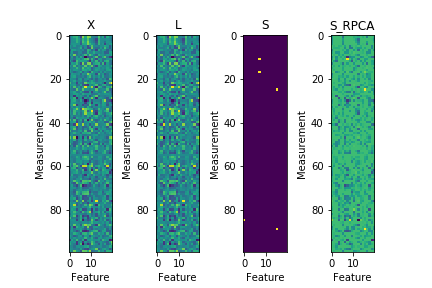
\includegraphics[width=.9\linewidth]{{images/new_7-13-2020/runRPCAAnomalyTest_images_m_200_n_20_k_6_numAnoms_10_sizeAnoms_0.001000}.png}
    \end{subfigure}
    \begin{subfigure}{.45\textwidth}
    \centering
    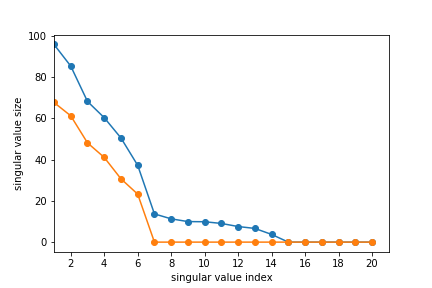
\includegraphics[width=.9\linewidth]{{images/new_7-13-2020/runRPCAAnomalyTest_singular_values_m_200_n_20_k_6_numAnoms_10_sizeAnoms_0.001000}.png}
    \end{subfigure}
    \caption{An easy example of RPCA with $10$ anomalies, each of size $50$.}
    \label{fig:m_200_n_20_k_6_numAnoms_10_sizeAnoms_0.001000}
\end{figure}

\todo{RCP: The labels for fig 5-8 should all be different.  Are they all needed: SHoudl we only included the hardest case it does well on and the simpliest one it doesn't poorly on?  Also, the blue and orange curves are incorrect (code error) and need legends.}

\begin{figure}
    \begin{subfigure}{.45\textwidth}
    \centering
    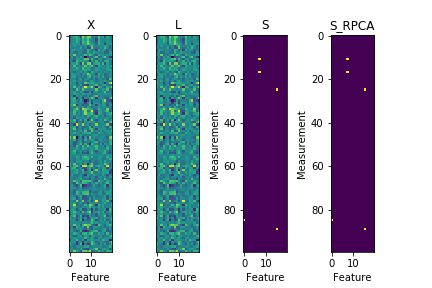
\includegraphics[width=.9\linewidth]{{images/new_7-13-2020/runRPCAAnomalyTest_images_m_200_n_20_k_6_numAnoms_10_sizeAnoms_1.000000}.png}
    \end{subfigure}
    \begin{subfigure}{.45\textwidth}
    \centering
    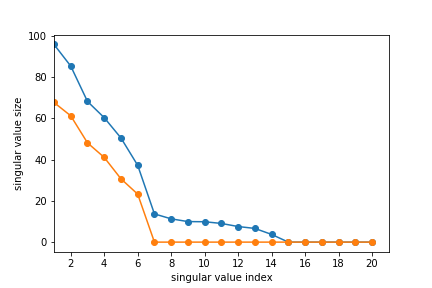
\includegraphics[width=.9\linewidth]{{images/new_7-13-2020/runRPCAAnomalyTest_singular_values_m_200_n_20_k_6_numAnoms_10_sizeAnoms_1.000000}.png}
    \end{subfigure}
    \caption{An easy example of RPCA with $10$ anomalies, each of size $50$.}
    \label{fig:m_200_n_20_k_6_numAnoms_10_sizeAnoms_1.000000}
\end{figure}

\begin{figure}
    \begin{subfigure}{.45\textwidth}
    \centering
    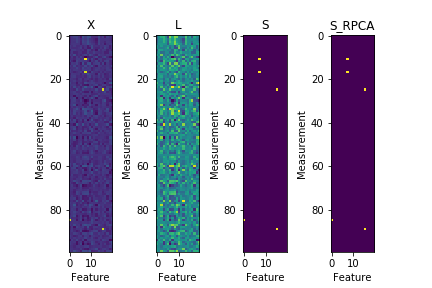
\includegraphics[width=.9\linewidth]{{images/new_7-13-2020/runRPCAAnomalyTest_images_m_200_n_20_k_6_numAnoms_10_sizeAnoms_50.000000}.png}
    \end{subfigure}
    \begin{subfigure}{.45\textwidth}
    \centering
    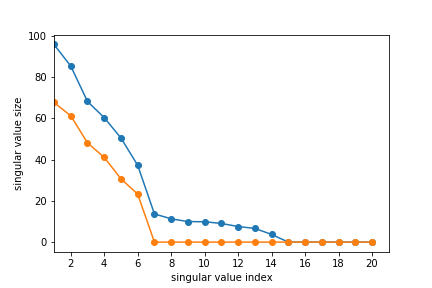
\includegraphics[width=.9\linewidth]{{images/new_7-13-2020/runRPCAAnomalyTest_singular_values_m_200_n_20_k_6_numAnoms_10_sizeAnoms_50.000000}.png}
    \end{subfigure}
    \caption{An easy example of RPCA with $10$ anomalies, each of size $50$.}
    \label{fig:m_200_n_20_k_6_numAnoms_10_sizeAnoms_50.000000}
\end{figure}

\begin{figure}
    \begin{subfigure}{.45\textwidth}
    \centering
    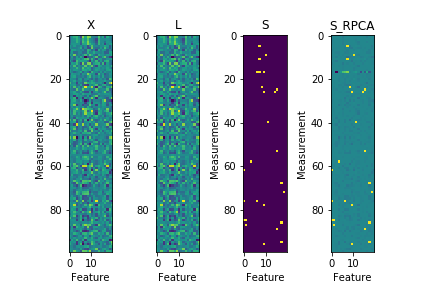
\includegraphics[width=.9\linewidth]{{images/new_7-13-2020/runRPCAAnomalyTest_images_m_200_n_20_k_6_numAnoms_50_sizeAnoms_0.010000}.png}
    \end{subfigure}
    \begin{subfigure}{.45\textwidth}
    \centering
    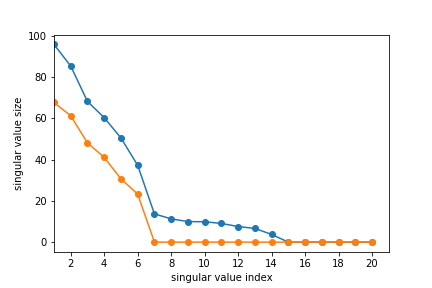
\includegraphics[width=.9\linewidth]{{images/new_7-13-2020/runRPCAAnomalyTest_singular_values_m_200_n_20_k_6_numAnoms_50_sizeAnoms_0.010000}.png}
    \end{subfigure}
    \caption{A difficult example of RPCA with $50$ anomalies, each of size $0.01$.  Note, even with many anomalies RPCA does a good job.}
    \label{fig:m_200_n_20_k_6_numAnoms_50_sizeAnoms_0.010000}
\end{figure}

\begin{figure}
    \begin{subfigure}{.45\textwidth}
    \centering
    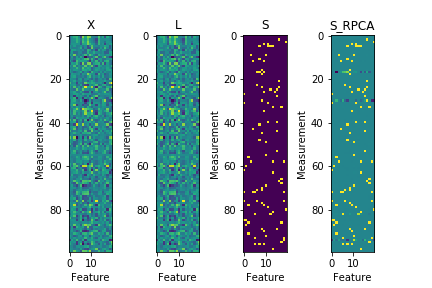
\includegraphics[width=.9\linewidth]{{images/new_7-13-2020/runRPCAAnomalyTest_images_m_200_n_20_k_6_numAnoms_200_sizeAnoms_0.100000}.png}
    \end{subfigure}
    \begin{subfigure}{.45\textwidth}
    \centering
    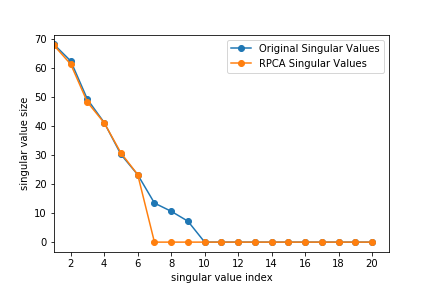
\includegraphics[width=.9\linewidth]{{images/new_7-13-2020/runRPCAAnomalyTest_singular_values_m_200_n_20_k_6_numAnoms_200_sizeAnoms_0.100000}.png}
    \end{subfigure}
    \caption{A difficult example of RPCA with $200$ anomalies, each of size $0.1$.}
    \label{fig:m_200_n_20_k_6_numAnoms_200_sizeAnoms_0.100000}
\end{figure}

%%%%%%%%%%%%%%%%%%%%%%%%%%%%%%%%%%%%%%%%%%%%%%%%%%%%%%%%%%%%%%%%

The key results of our work can be found in Figures \ref{fig:error_PCA_prediction_without_RPCA}, \ref{fig:error_PCA_prediction_with_RPCA_first}, \ref{fig:error_SPCA_prediction_without_RPCA_first}, \ref{fig:error_SPCA_prediction_without_RPCA_first_selected}, \ref{fig:error_SPCA_prediction_with_RPCA_first}, and \ref{fig:error_SPCA_prediction_with_RPCA_first_selected}.
Figure \ref{fig:error_PCA_prediction_without_RPCA} shows a purely PCA based prediction.  Besides requiring all of the original predictors to compute, the anomalies in the training and testing data cause many errors in reconstruction.  
Figure \ref{fig:error_PCA_prediction_with_RPCA_first} shows a purely SPCA based prediction.  Again, the anomalies in the testing data cause many errors in the reconstruction.
Figures \ref{fig:error_SPCA_prediction_without_RPCA_first} and \ref{fig:error_SPCA_prediction_without_RPCA_first_selected} show a PCA prediction after an RPCA preprocessing.  While superior to the pure PCA reconstruction, anomalies in the testing data still cause substantial errors. 
\todo[color=yellow]{LS: It seems that FIg 14 and 15 are the big achievement: Some in a quantitative form this should be summarized in the intro}
Figures \ref{fig:error_SPCA_prediction_with_RPCA_first} and \ref{fig:error_SPCA_prediction_with_RPCA_first_selected} show an SPCA prediction after an RPCA preprocessing.  In this case both the low-rank background and the anomalies are exactly recovered, up to the error arising in the RPCA optimization.

\begin{figure}
    \centering
    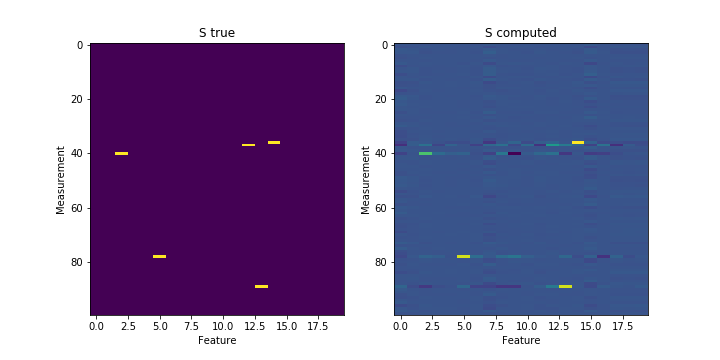
\includegraphics[width=0.45\textwidth]{{images/new_7-13-2020/short_test_S_title_PCA_prediction_without_RPCA_first_m_200_n_20_k_6_noiseSize_0.000000_numAnoms_10_sizeAnoms_1.000000}.png}
    \caption{A PCA prediction without RPCA first.  Note that both columns and rows have noise.}
    \label{fig:error_PCA_prediction_without_RPCA}
\end{figure}

\begin{figure}
    \centering
    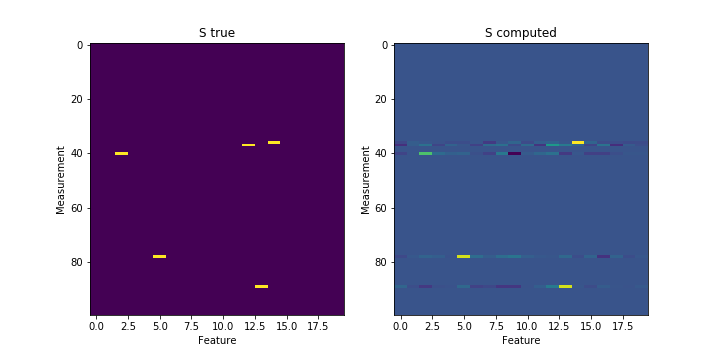
\includegraphics[width=0.45\textwidth]{{images/new_7-13-2020/short_test_S_title_PCA_prediction_with_RPCA_first_m_200_n_20_k_6_noiseSize_0.000000_numAnoms_10_sizeAnoms_1.000000}.png}
    \caption{A PCA prediction with RPCA first.  Note that only the rows have noise where there are anomalies in the testing data.}
    \label{fig:error_PCA_prediction_with_RPCA_first}
\end{figure}

\begin{figure}
    \centering
    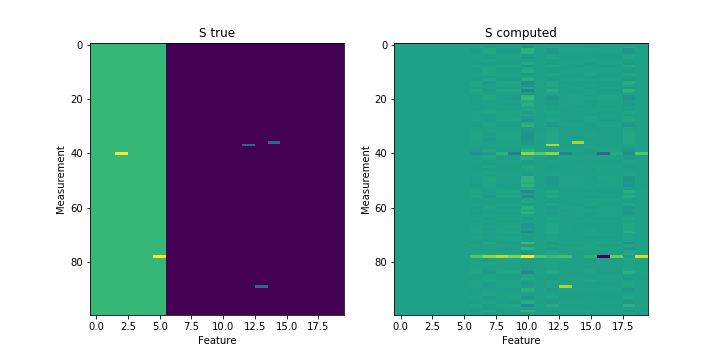
\includegraphics[width=0.45\textwidth]{{images/new_7-13-2020/short_test_S_title_SPCA_prediction_without_RPCA_first_m_200_n_20_k_6_noiseSize_0.000000_numAnoms_10_sizeAnoms_1.000000}.png}
    \caption{An SPCA prediction without RPCA first.  Note that, similar to PCA without RPCA, both columns and rows are incorrect because of anomalies in the training data.}
    \label{fig:error_SPCA_prediction_without_RPCA_first}
\end{figure}

\begin{figure}
    \centering
    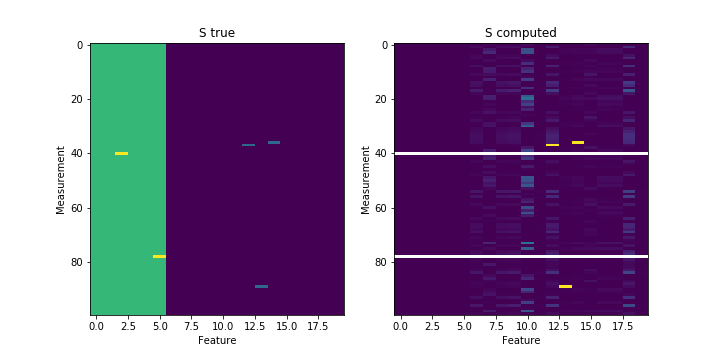
\includegraphics[width=0.45\textwidth]{{images/new_7-13-2020/short_test_S_title_SPCA_prediction_without_RPCA_first_selected_m_200_n_20_k_6_noiseSize_0.000000_numAnoms_10_sizeAnoms_1.000000}.png}
    \caption{An SPCA prediction without RPCA first.  Note that, similar to PCA without RPCA, both columns and rows are incorrect because of anomalies in the training data.  In this figure we emphasize the errors caused by training data by removing the rows with anomalies in the testing data.}
    \label{fig:error_SPCA_prediction_without_RPCA_first_selected}
\end{figure}


% \begin{figure*}
% \begin{subfigure}{.45\textwidth}
%     \centering
%     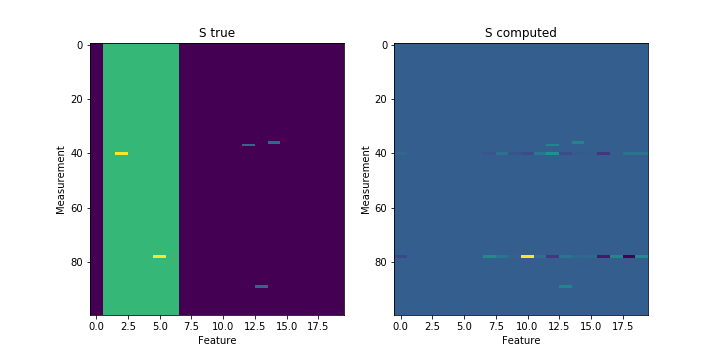
\includegraphics[width=0.9\textwidth]{{images/new_7-13-2020/short_test_S_title_SPCA_prediction_with_RPCA_first_m_200_n_20_k_6_noiseSize_0.000000_numAnoms_10_sizeAnoms_1.000000}.png}
%     \caption{An SPCA prediction without RPCA first.  Note that, similar to PCA with RPCA, both only rows are incorrect because of anomalies in the testing data.}
%     \label{fig:error_SPCA_prediction_with_RPCA_first}
% \end{subfigure}
% \begin{subfigure}{.45\textwidth}
%     \centering
%     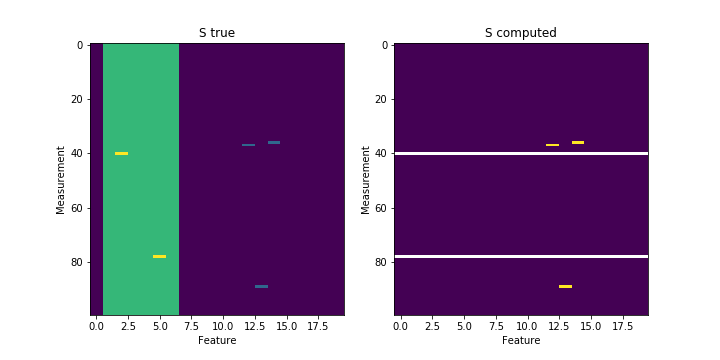
\includegraphics[width=0.9\textwidth]{{images/new_7-13-2020/short_test_S_title_SPCA_prediction_with_RPCA_first_selected_m_200_n_20_k_6_noiseSize_0.000000_numAnoms_10_sizeAnoms_1.000000}.png}
%     \caption{An SPCA prediction without RPCA first.  Note that, similar to PCA with RPCA, both only rows are incorrect because of anomalies in the testing data.  In this figure we show that the anomalies are exactly recovered in by removing the rows with anomalies in the testing data.}
%     \label{fig:error_SPCA_prediction_with_RPCA_first_selected}
% \end{subfigure}
% \end{figure*}

\begin{figure}
    \centering
    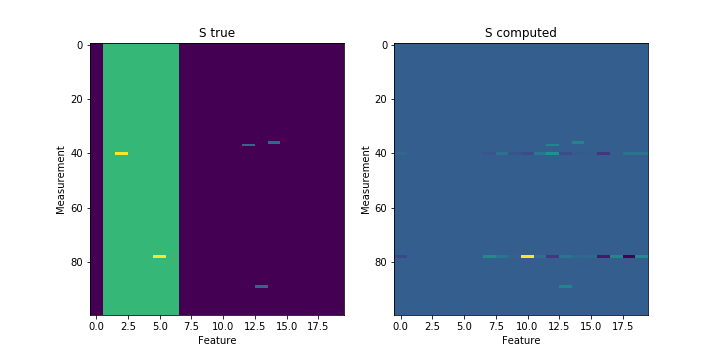
\includegraphics[width=0.45\textwidth]{{images/new_7-13-2020/short_test_S_title_SPCA_prediction_with_RPCA_first_m_200_n_20_k_6_noiseSize_0.000000_numAnoms_10_sizeAnoms_1.000000}.png}
    \caption{An SPCA prediction without RPCA first.  Note that, similar to PCA with RPCA, both only rows are incorrect because of anomalies in the testing data.}
    \label{fig:error_SPCA_prediction_with_RPCA_first}
\end{figure}
\begin{figure}
    \centering
    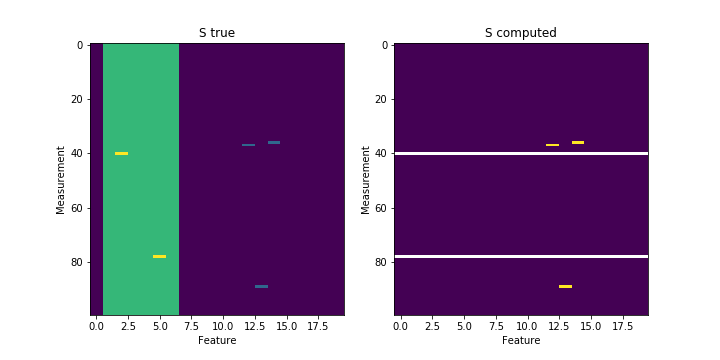
\includegraphics[width=0.45\textwidth]{{images/new_7-13-2020/short_test_S_title_SPCA_prediction_with_RPCA_first_selected_m_200_n_20_k_6_noiseSize_0.000000_numAnoms_10_sizeAnoms_1.000000}.png}
    \caption{An SPCA prediction without RPCA first.  Note that, similar to PCA with RPCA, both only rows are incorrect because of anomalies in the testing data.  In this figure we show that the anomalies are exactly recovered in by removing the rows with anomalies in the testing data.}
    \label{fig:error_SPCA_prediction_with_RPCA_first_selected}
\end{figure}


%%%%%%%%%%%%%%%%%%%%%%%%%%%%%%%%%%%%%%%%%%%%%%%%%%%%%%%%%%%%%%%%

% \begin{figure}
%     \centering
%     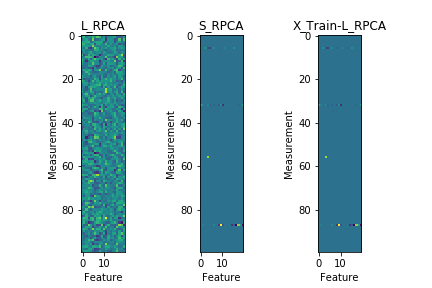
\includegraphics[width=0.45\textwidth]{{images/new_7-13-2020/short_train_S_m_200_n_20_k_10_noiseSize_0.000000_numAnoms_10_sizeAnoms_1.000000}.png}
%     \caption{Caption}
%     \label{fig:my_label}
% \end{figure}

%%%%%%%%%%%%%%%%%%%%%%%%%%%%%%%%%%%%%%%%%%%%%%%%%%%%%%%%%%%%%%%%

Figure \ref{fig:real_data} shows the results of our methodologies running on real healthcare provided data.  As we do not know where the true anomalies, if any occur, we test our methodology by adding anomalies of our own.  We then tune $\lambda$ to the largest value for which these anomalies are detected in $S$.  As one may observe, our method exactly detects both our added anomalies as well as additional \emph{true} anomalies in the real-world data.

\begin{figure*}
    \centering
    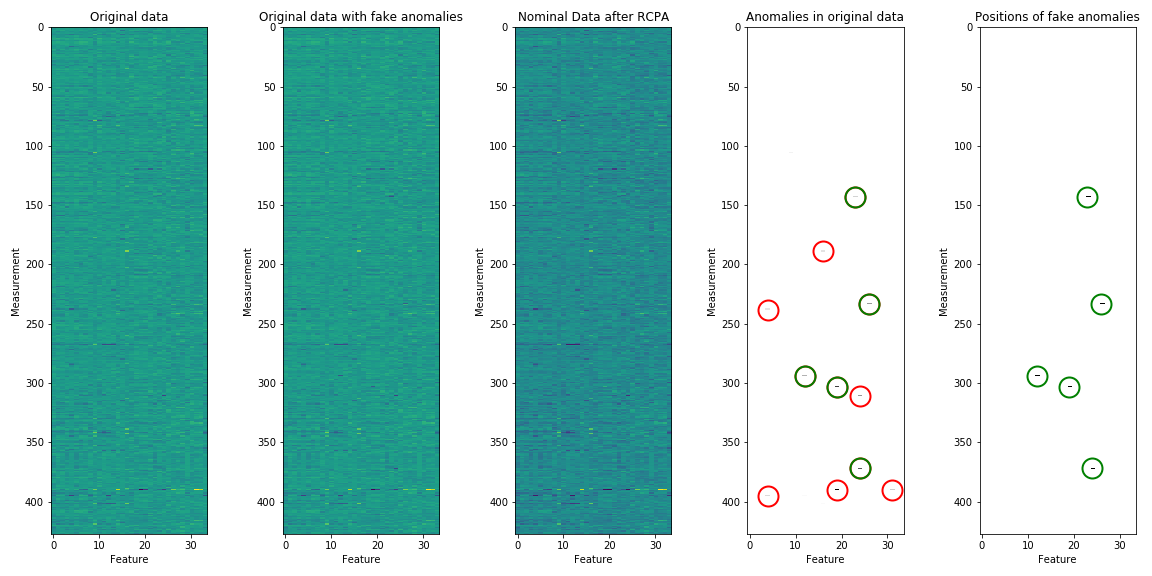
\includegraphics[width=0.8\textwidth]{images/new_7-13-2020/real_data.png}
    \caption{An example of RPCA analysis on real data.   We add anomalies of our own and choose the smallest $\lambda$ that recovers our added anomalies.  The entries in red circles are anomalies in the actual data.}
    \label{fig:real_data}
\end{figure*}

\todo[color=yellow]{LS:  What do we learn from fig 16 in terms of recommended policy?
We should summarize that we can recover placed anomalies in the real data in the intro. Also, summarize recommendation.}
\todo{RCP:  I think we need another graphic to support the claim that we believe using our analysis that we only need X metrics and that the impact of that will be Y.  For example a singular value plot for the real data.  However, I am not sure this is very clear.}


% \begin{figure}[H]
%     \centering
%     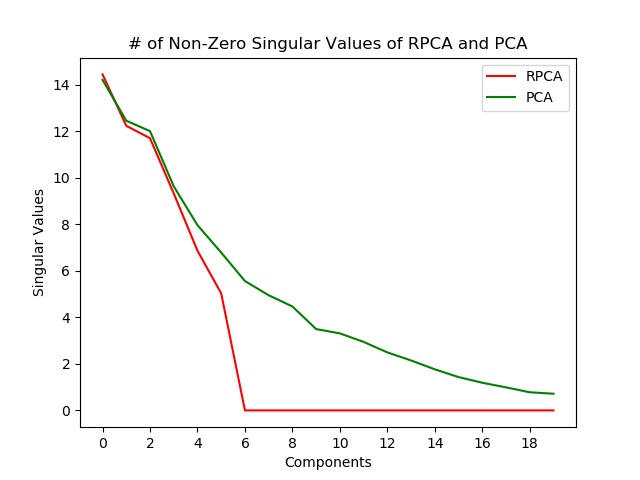
\includegraphics[width=50mm, scale=0.5]{Singular_Value_Plot_Test_120AnomSize5.jpg}
%     \caption{Singular Value comparison for PCA and RPCA on synthetic data with 3 percent anomalies of size 5}
%     \label{fig:singvaltrain1205}
% \end{figure}

% \begin{figure}[H]
%     \centering
%     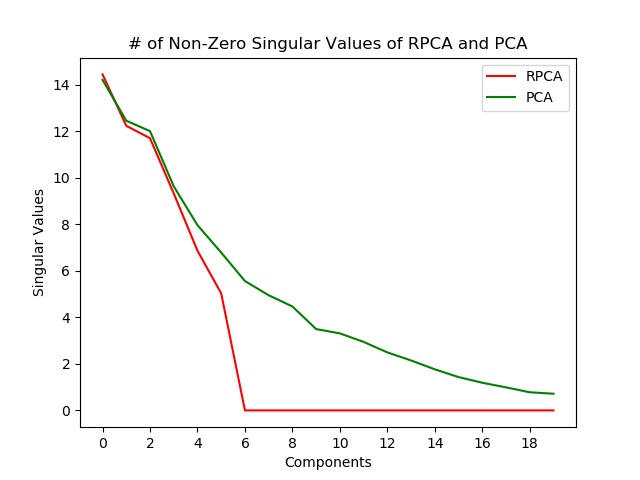
\includegraphics[width=50mm, scale=0.5]{Singular_Value_Plot_Test_120AnomSize5.jpg}
%     \caption{Singular Value comparison for PCA and RPCA on synthetic data with 3 percent anomalies of size 5}
%     \label{fig:singvaltrain1205}
% \end{figure}

% \begin{figure}[H]
% \begin{minipage}[b]{0.45\linewidth}
%     \centering
%     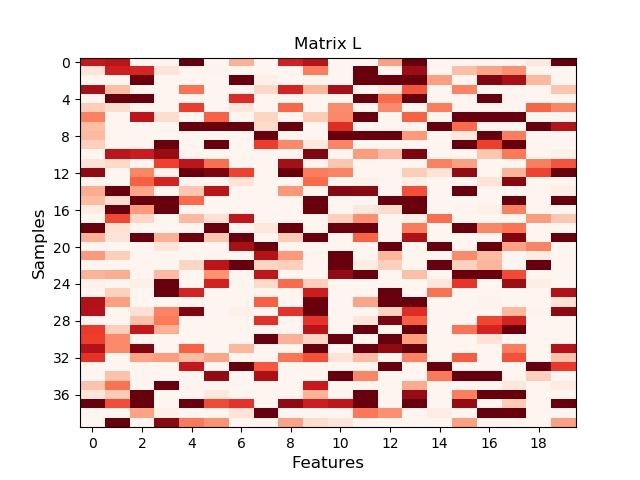
\includegraphics[width=45mm, scale=0.5]{L_120AnomSize5.jpg}
%     \caption{Low-Rank Matrix resulting from RPCA on synthetic data with 3 percent anomalies of size 5}
%     \label{fig:Ltrain1205}
% \end{minipage}
% \quad
% \begin{minipage}[b]{0.45\linewidth}
%     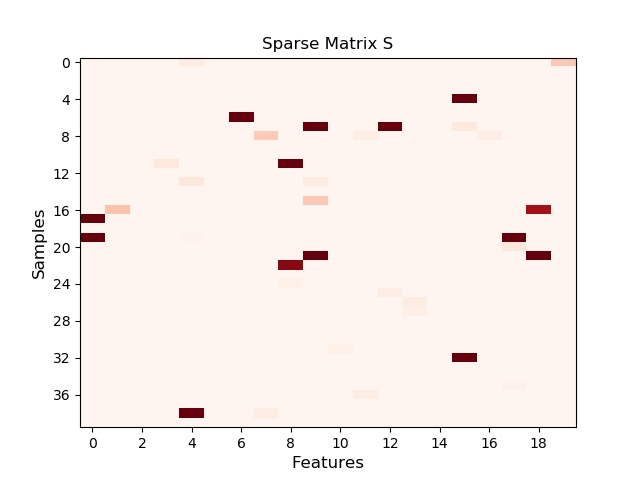
\includegraphics[width=45mm, scale=0.5]{S_120AnomSize5.jpg}
%     \caption{Sparse Matrix resulting from RPCA on synthetic data with 3 percent anomalies of size 5}
%     \label{fig:Strain1205}
% \end{minipage}
% \end{figure}

% \begin{figure}[H]
% \begin{minipage}[b]{0.45\linewidth}
%     \centering

%     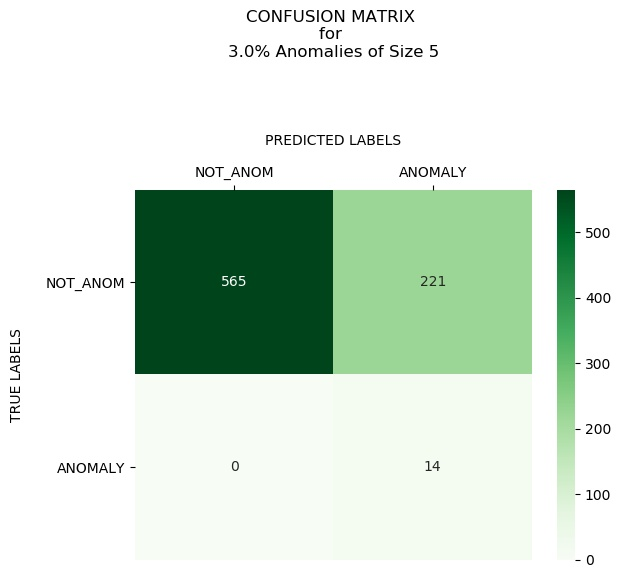
\includegraphics[width=50mm, scale=0.5]{cmPCATest_120AnomSize5.jpg}
%     \caption{Confusion Matrix resulting from PCA on synthetic data with 3 percent anomalies of size 5}
%     \label{fig::CMtrainPCA1205}
% \end{minipage}
% \quad
% \begin{minipage}[b]{0.45\linewidth}
%     \centering
%     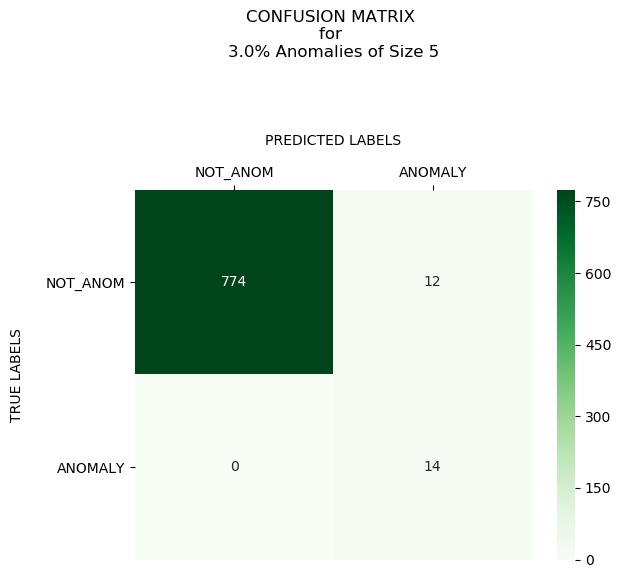
\includegraphics[width=50mm, scale=0.5]{cmRPCATest_120AnomSize5.jpg}
%     \caption{Confusion Matrix resulting from RPCA on synthetic data with 3 percent anomalies of size 5}
%     \label{fig::CMtrainRPCA125}
% \end{minipage}
% \end{figure}

% % Insert Figures for three percent anomalies size 10

% \begin{figure}[H]
%     \centering
%     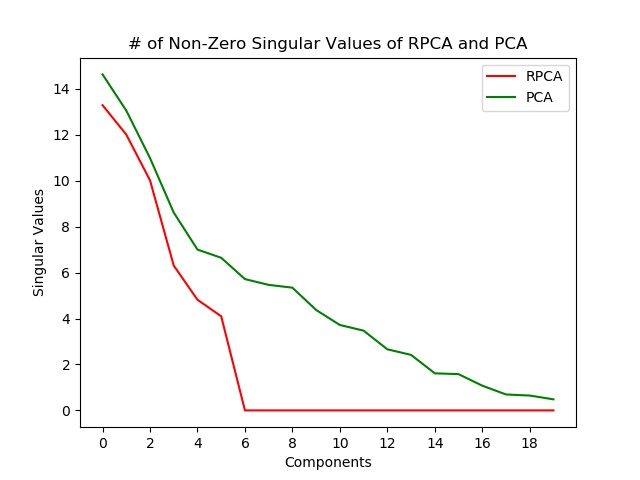
\includegraphics[width=50mm, scale=0.5]{Singular_Value_Plot_Test_120AnomSize10.jpg}
%     \caption{Singular Value comparison for PCA and RPCA on synthetic data with 3 percent anomalies of size 10}
%     \label{fig:singvaltrain12010}
% \end{figure}
% \begin{figure}[H]
% \begin{minipage}[b]{0.45\linewidth}
%     \centering
%     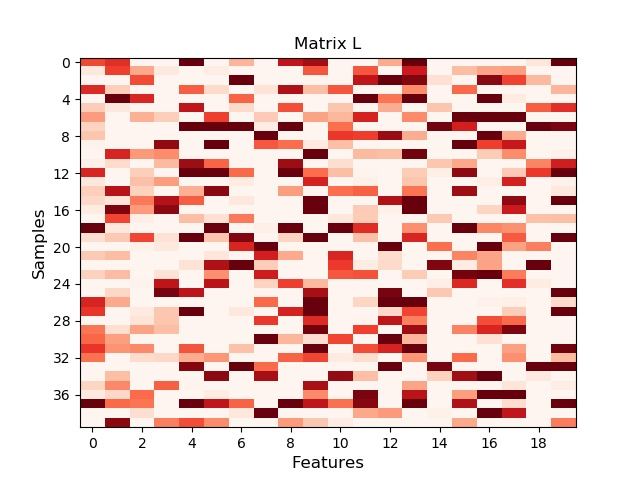
\includegraphics[width=45mm, scale=0.5]{L_120AnomSize10.jpg}
%     \caption{Low-Rank Matrix resulting from RPCA on synthetic data with 3 percent anomalies of size 10}
%     \label{fig:Ltrain12010}
% \end{minipage}
% \quad
% \begin{minipage}[b]{0.45\linewidth}
%     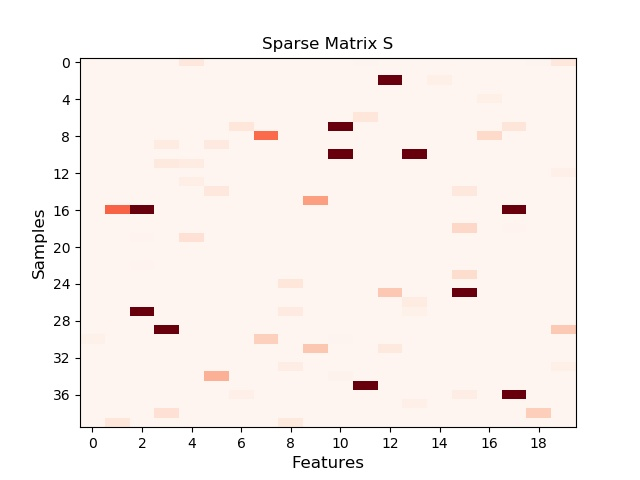
\includegraphics[width=45mm, scale=0.5]{S_120AnomSize10.jpg}
%     \caption{Sparse Matrix resulting from RPCA on synthetic data with 3 percent anomalies of size 10}
%     \label{fig:Strain12010}
% \end{minipage}
% \end{figure}

% \begin{figure}[H]
% \begin{minipage}[b]{0.45\linewidth}
%     \centering

%     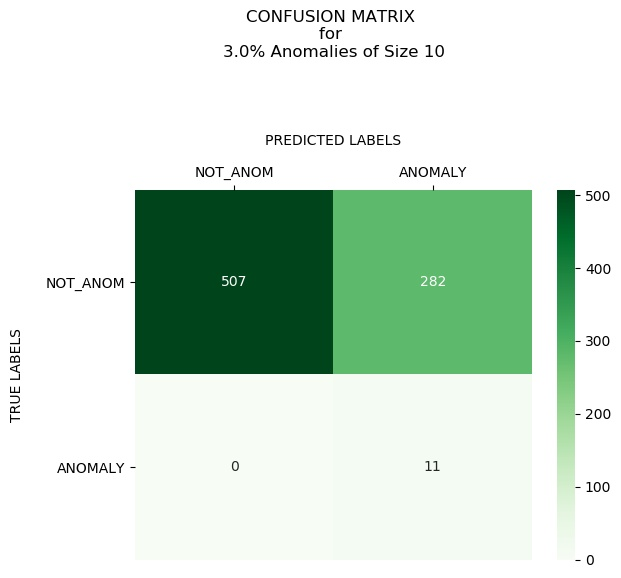
\includegraphics[width=50mm, scale=0.5]{cmPCATest_120AnomSize10.jpg}
%     \caption{Confusion Matrix resulting from PCA on synthetic data with 3 percent anomalies of size 10}
%     \label{fig::CMtrainPCA12010}
% \end{minipage}
% \quad
% \begin{minipage}[b]{0.45\linewidth}
%     \centering
%     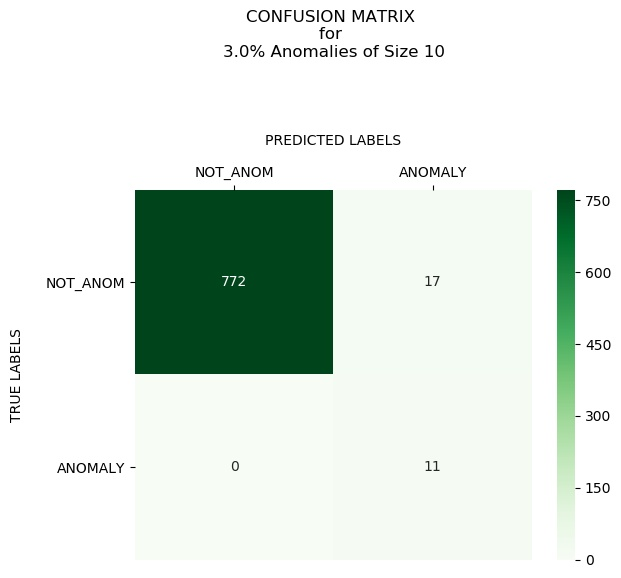
\includegraphics[width=50mm, scale=0.5]{cmRPCATest_120AnomSize10.jpg}
%     \caption{Confusion Matrix resulting from RPCA on synthetic data with 3 percent anomalies of size 10}
%     \label{fig::CMtrainRPCA12010}
% \end{minipage}
% \end{figure}

% % Insert Figures for ten percent anomalies size 5

% \begin{figure}[H]
%     \centering
%     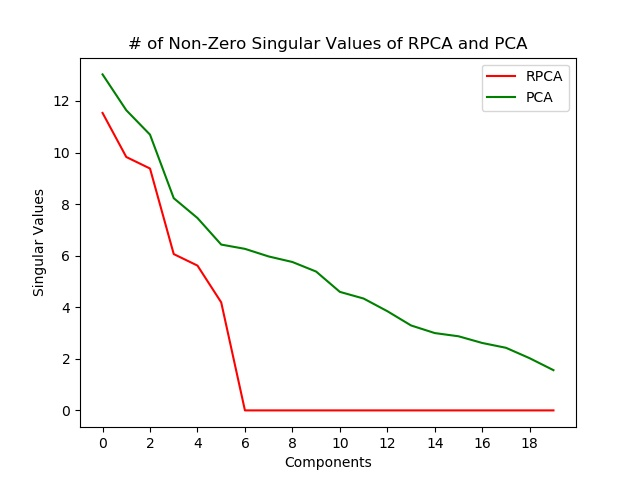
\includegraphics[width=50mm, scale=0.5]{Singular_Value_Plot_Test_400AnomSize5.jpg}
%     \caption{Singular Value comparison for PCA and RPCA on synthetic data with 10 percent anomalies of size 5}
%     \label{fig:singvaltrain4005}
% \end{figure}
% \begin{figure}[H]
% \begin{minipage}[b]{0.45\linewidth}
%     \centering
%     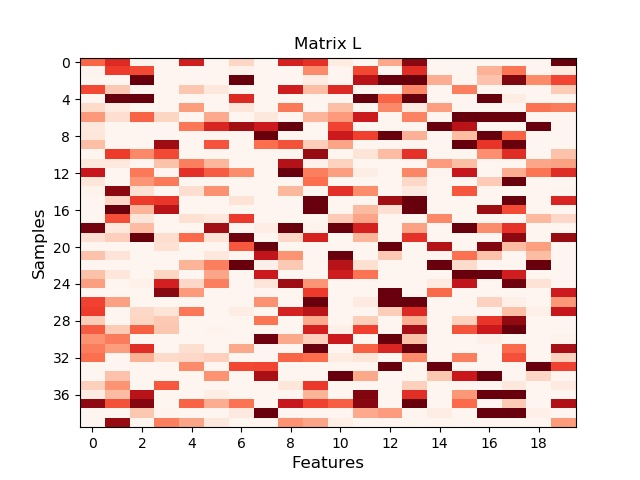
\includegraphics[width=45mm, scale=0.5]{L_400AnomSize5.jpg}
%     \caption{Low-Rank Matrix resulting from RPCA on synthetic data with 10 percent anomalies of size 5}
%     \label{fig:Ltrain4005}
% \end{minipage}
% \quad
% \begin{minipage}[b]{0.45\linewidth}
%     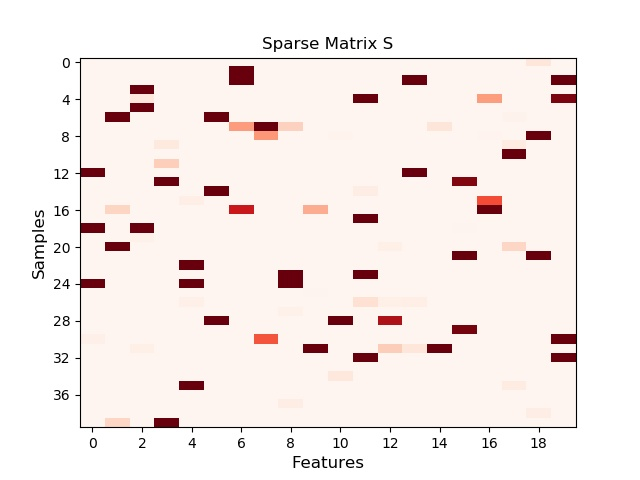
\includegraphics[width=45mm, scale=0.5]{S_400AnomSize5.jpg}
%     \caption{Sparse Matrix resulting from RPCA on synthetic data with 10 percent anomalies of size 5}
%     \label{fig:Strain4005}
% \end{minipage}
% \end{figure}

% \begin{figure}[H]
% \begin{minipage}[b]{0.45\linewidth}
%     \centering

%     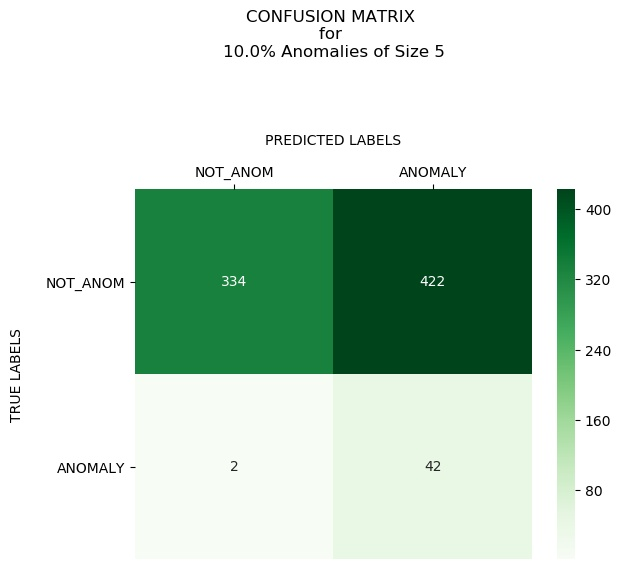
\includegraphics[width=50mm, scale=0.5]{cmPCATest_400AnomSize5.jpg}
%     \caption{Confusion Matrix resulting from PCA on synthetic data with 10 percent anomalies of size 5}
%     \label{fig::CMtrainPCA4005}
% \end{minipage}
% \quad
% \begin{minipage}[b]{0.45\linewidth}
%     \centering
%     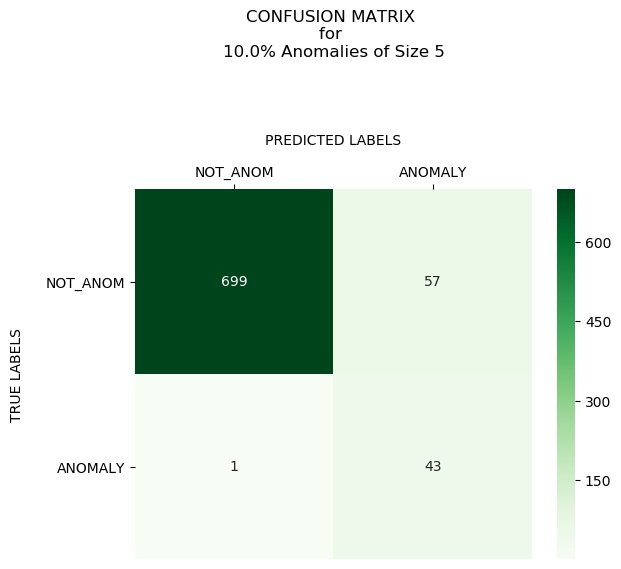
\includegraphics[width=50mm, scale=0.5]{cmRPCATest_400AnomSize5.jpg}
%     \caption{Confusion Matrix resulting from RPCA on synthetic data with 10 percent anomalies of size 5}
%     \label{fig::CMtrainRPCA4005}
% \end{minipage}
% \end{figure}

% % Insert Figures for ten percent anomalies size 10

% \begin{figure}[H]
%     \centering
%     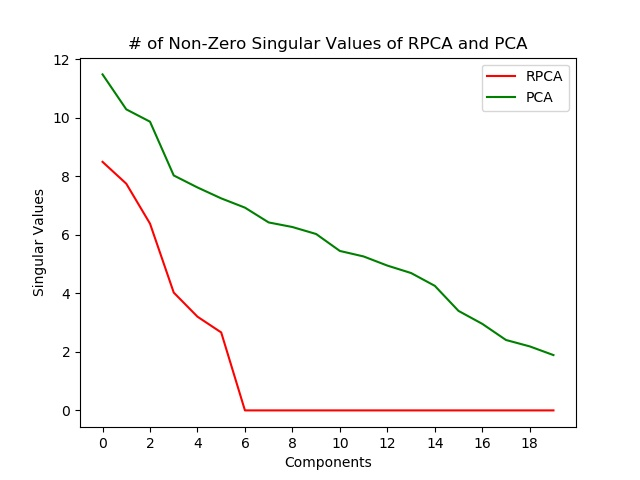
\includegraphics[width=50mm, scale=0.5]{Singular_Value_Plot_Test_400AnomSize10.jpg}
%     \caption{Singular Value comparison for PCA and RPCA on synthetic data with 10 percent anomalies of size 10}
%     \label{fig:singvaltrain40010}
% \end{figure}
% \begin{figure}[H]
% \begin{minipage}[b]{0.45\linewidth}
%     \centering
%     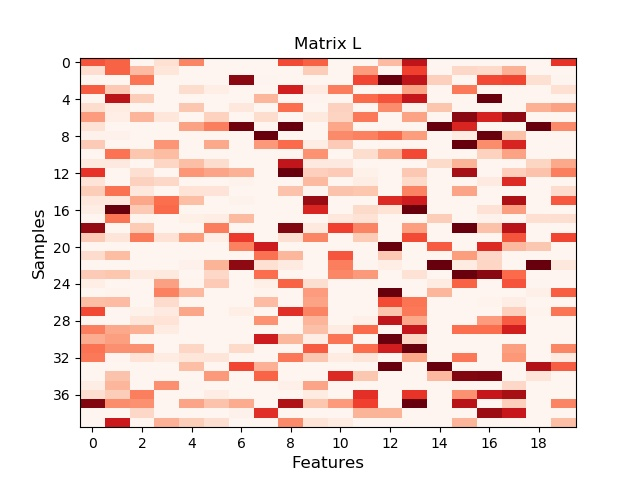
\includegraphics[width=45mm, scale=0.5]{L_400AnomSize10.jpg}
%     \caption{Low-Rank Matrix resulting from RPCA on synthetic data with 10 percent anomalies of size 10}
%     \label{fig:Ltrain40010}
% \end{minipage}
% \quad
% \begin{minipage}[b]{0.45\linewidth}
%     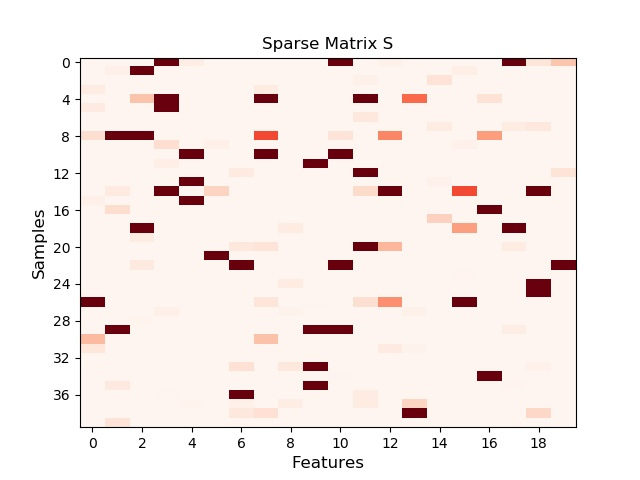
\includegraphics[width=45mm, scale=0.5]{S_400AnomSize10.jpg}
%     \caption{Sparse Matrix resulting from RPCA on synthetic data with 10 percent anomalies of size 10}
%     \label{fig:Strain40010}
% \end{minipage}
% \end{figure}

% \begin{figure}[H]
% \begin{minipage}[b]{0.45\linewidth}
%     \centering

%     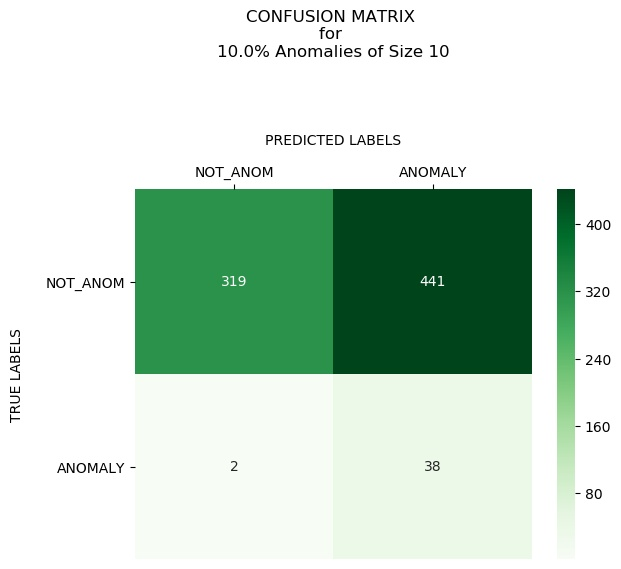
\includegraphics[width=50mm, scale=0.5]{cmPCATest_400AnomSize10.jpg}
%     \caption{Confusion Matrix resulting from PCA on synthetic data with 10 percent anomalies of size 10}
%     \label{fig::CMtrainPCA40010}
% \end{minipage}
% \quad
% \begin{minipage}[b]{0.45\linewidth}
%     \centering
%     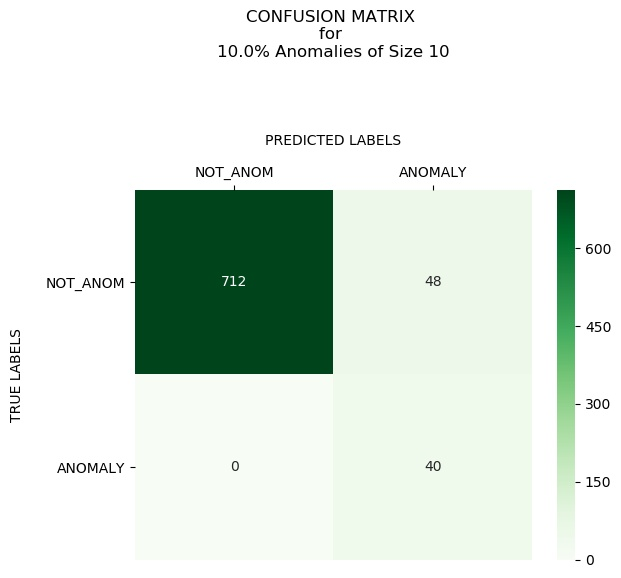
\includegraphics[width=50mm, scale=0.5]{cmRPCATest_400AnomSize10.jpg}
%     \caption{Confusion Matrix resulting from RPCA on synthetic data with 10 percent anomalies of size 10}
%     \label{fig::CMtrainRPCA40010}
% \end{minipage}
% \end{figure}

% \todo[inline]{Add MSE plots of outliers against error plot data csv files}
% \todo[inline]{Add results for Deon's combinatorial approach}
\todo{RCP: Add approach for real data}
% \todo[inline]{Do Paffenroth insertions: add anomalies and show that we found them}
% \todo[inline]{Add results for real data: What does PCA/RPCA/Gurobi find}

\section{Conclusions}

This work presents a new research path to explore how modern optimization methods can help complement medical and policy judgment when seeking to reduce health metric burdens.  In particular, our methodology recommends  the minimum selection of health metrics from a proposed set of candidates when there is reason to expect confounding measurement errors in the data.

In particular, empirical examples on synthetic data show our approach was the only method tested herein that found all possible anomalies with no false alarms and perfectly computed the required reduced number of metrics needed without appreciable loss of information. 

 

\todo[color=yellow]{LS: Conclusions: I think we should be more assertive: We developed empirical evidence that using new modern optimization methods can be effective at complementing }

\section{Acknowledgment}
The authors wish to thank Dr. Allen Leavens, (MITRE) for introducing us to the challenges of health reporting burdens as well as the introducing us to the Center for Medicare and Medicaid Services (CMS)'s public use dataset related to the Shared Saving Program Accountable Care Organization (ACO).  

\clearpage



\todo[color=yellow]{LS:  Ask Melanie to proof complete document}

\bibliographystyle{IEEEtran}
\bibliography{ICMLA}

\newpage
\listoftodos[Notes]
\end{document}
